% Modified based on Xiaoming Sun's template and https://www.overleaf.com/latex/templates/cs6780-assignment-template/hgjyygbykvrf

\documentclass[a4 paper,12pt]{article}
\usepackage[inner=2.0cm,outer=2.0cm,top=2.0cm,bottom=2.0cm]{geometry}
\linespread{1.1}
\usepackage{setspace}
\usepackage[rgb]{xcolor}
\usepackage{verbatim}
\usepackage{subcaption}
\usepackage{fancyhdr}
\usepackage{fullpage}
\usepackage[colorlinks=true, urlcolor=blue, linkcolor=blue, citecolor=blue]{hyperref}
\usepackage{booktabs}
\usepackage{amsmath,amsfonts,amsthm,amssymb}
\usepackage[shortlabels]{enumitem}
\usepackage{setspace}
\usepackage{extramarks}
\usepackage{soul,color}
\usepackage{graphicx,float,wrapfig}
\newcommand{\homework}[3]{
	\pagestyle{myheadings}
	\thispagestyle{plain}
	\newpage
	\setcounter{page}{1}
	\noindent
	\begin{center}
		\framebox{
			\vbox{\vspace{2mm}
				\hbox to 6.28in { {\bf Deep Learning \hfill} {\hfill {\rm #2} {\rm #3}} }
				\vspace{4mm}
				\hbox to 6.28in { {\Large \hfill #1  \hfill} }
				\vspace{3mm}}
		}
	\end{center}
	\vspace*{4mm}
}
\newcommand\numberthis{\addtocounter{equation}{1}\tag{\theequation}}
\usepackage[english]{babel}
%Includes "References" in the table of contents
\usepackage[nottoc]{tocbibind}
\begin{document}
	\homework{Homework 4}{2023040163}{Zhao Han Hong}
	
	\section*{1 True or False Questions}
	\section*{Problem 1}

	False.
	\section*{Problem 2}

	True.

	\section*{Problem 3}

	False.

	\section*{Problem 4}

	False.

	\section*{2 Q \& A}
\newcommand*{\norm}[1]{\left|\left|#1\right|\right|}
\newcommand*{\E}[0]{\mathbb{E}}
\newcommand*{\p}[0]{\mathbb{P}}
\section*{Problem 5}

In the E step, $\theta$ is fixed, so the equivalent objective is
\[
F({\theta^{(t)}},q)=\sum_z q(z)\log p_{\theta^{(t)}}(x,z) - \sum_z q(z) \log q(z)=\sum_z q(z)\log \frac{p_{\theta^{(t)}}(x,z)}{q(z)}.
\]  Since $\log x$ is a concave function, we have that
\[
\sum_z q(z)\log \frac{p_{\theta^{(t)}}(x,z)}{q(z)} \le \log \sum_z q(z) \frac{p_{\theta^{(t)}}(x,z)}{q(z)} = \log \sum_z p_{\theta^{(t)}}(x,z) = \log p_{\theta^{(t)}}(x),
\] and the equation holds if and only if $q(z)=p_{\theta^{(t)}}(z|x)$. Thus, after the E step, the objective becomes
\[
F(\theta,q^{(t)})=\log \sum_z p_{\theta^{(t)}}(x,z) ,
\] which is exactly the target in the original M step. Thus, we are done.

\section*{Problem 6}
\paragraph{1.} We can use the definition to compute:
\begin{align*}
&\quad \text{KL}(\mathcal{N}_0||\mathcal{N}_1)\\
&=\int \frac{1}{(\sqrt{2\pi})^d\sqrt{\det \Sigma_0}}\exp\left(-\frac{1}{2}(x-\mu_0)^T\Sigma_0^{-1}(x-\mu_0)\right)\cdot \frac{1}{2}\Big(\ln \frac{\det \Sigma_1}{\det \Sigma_0}-(x-\mu_0)^T\Sigma_0^{-1}(x-\mu_0)\\
& \qquad +(x-\mu_1)^T\Sigma_1^{-1}(x-\mu_1)\Big)dx\\
&=\frac{1}{2}\left(\ln \frac{|\Sigma_1|}{|\Sigma_0|}-\text{tr}\left((\Sigma_0^{-1})^T\Sigma_0\right)+(\mu_0-\mu_1)^T\Sigma_1^{-1}(\mu_0-\mu_1)+\text{tr}\left(\Sigma_1^{-1}\Sigma_0\right)\right)\\
&=\frac{1}{2}\left(\ln \frac{|\Sigma_1|}{|\Sigma_0|}-d+(\mu_0-\mu_1)^T\Sigma_1^{-1}(\mu_0-\mu_1)+\text{tr}\left(\Sigma_1^{-1}\Sigma_0\right)\right),
\end{align*} where we have used the fact that for a Gaussian distribution $\mathcal{N}(\mu,\Sigma)$, we have
\[
\E[(x_i-\mu_i)(x_j-\mu_j)]=\Sigma_{ij}
\]
\paragraph*{2.} Let the RHS$-$LHS be $f(\lambda)$. We can the take derivatives of $f(\lambda)$:
\begin{align*}
\quad f'(\lambda)&=\frac{d}{d\lambda}\Big[\lambda\sum_{y}p_1(y)\ln \frac{p_1(y)}{q_1(y)}+(1-\lambda)\sum_{y}p_2(y)\ln \frac{p_2(y)}{q_2(y)}\\
&\qquad -\sum_{y}(\lambda p_1(y)+(1-\lambda)p_2(y))\ln \frac{\lambda p_1(y)+(1-\lambda)p_2(y)}{\lambda q_1(y)+(1-\lambda)q_2(y)}\Big]\\
&= \sum_{y}\Big[p_1(y)\ln \frac{p_1(y)}{q_1(y)}-p_2(y)\ln \frac{p_2(y)}{q_2(y)}-\left(p_1(y)-p_2(y)\right)\left(1+\ln \frac{\lambda p_1(y)+(1-\lambda)p_2(y)}{\lambda q_1(y)+(1-\lambda)q_2(y)}\right)\\
&\qquad +(q_1(y)-q_2(y))\frac{\lambda p_1(y)+(1-\lambda)p_2(y)}{\lambda q_1(y)+(1-\lambda)q_2(y)}\Big];
\end{align*}
\begin{align*}
f''(\lambda)&=\sum_y\Big[ \left(-(p_1(y)-p_2(y))\frac{\lambda q_1(y)+(1-\lambda)q_2(y)}{\lambda p_1(y)+(1-\lambda)p_2(y)}+(q_1(y)-q_2(y))\right)\cdot \\
&\frac{(p_1(y)-p_2(y))(\lambda q_1(y)+(1-\lambda)q_2(y))-(q_1(y)-q_2(y))(\lambda p_1(y)+(1-\lambda)p_2(y))}{(\lambda q_1(y)+(1-\lambda)q_2(y))^2}\Big]\\
&=\sum_y\Big[\frac{p_2(y)q_1(y)-p_1(y)q_2(y)}{\lambda p_1(y)+(1-\lambda)p_2(y)} \frac{p_1(y)q_2(y)-p_2(y)q_1(y)}{(\lambda q_1(y)+(1-\lambda)q_2(y))^2}\Big]\\
&=-\sum_y\frac{(p_2(y)q_1(y)-p_1(y)q_2(y))^2}{(\lambda p_1(y)+(1-\lambda)p_2(y))(\lambda q_1(y)+(1-\lambda)q_2(y))^2}\le 0.
\end{align*} Thus, we can see that the minimal value of $f(\lambda)$ occurs at the boundary, i.e., $\lambda=0$ or $\lambda=1$. However, we can see that $f(0)=0$ and $f(1)=0$, so the minimal value of $f(\lambda)$ is 0. Thus, we are done.

\paragraph*{3.}
Here is the image.
\begin{figure}[H]
	\centering
	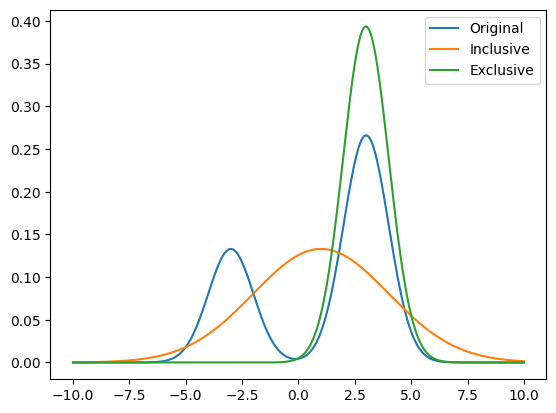
\includegraphics[width=0.5\textwidth]{./output.png}
	\label{fig:myfigure}
\end{figure}
(Side note: the figure shows that the inclusive KL captures all modes, and the exclusive KL only keeps the largest mode. Moreover, during the training process, I can notice that the exclusive KL loss gives a lot of local minima, since a learning rate smaller than 0.05 will make the model stay at a local minimum.)

\paragraph*{4.}
As stated in the problem, our objective is the KL divergence
\[
\text{KL}(p(z|x)||q(z|x))=\sum_z{p(z|x)}\log \frac{p(z|x)}{q(z|x)}.
\] Now, since we only consider optimizing $q(z|x)$, we can ignore the terms that do not depend on $q(z|x)$, and thus our objective becomes
\[
\text{Const}-\sum_z\frac{p(z,x)}{p(x)}\log q(z|x)=\text{Const}-\frac{1}{p(x)}\E_{z\sim p(z)}[p(x|z)\log q(z|x)].
\]

If we use this objective, the \textbf{pros} are that we can avoid the mode collapse problem, as the forward KL divergence include all possible modes. However, the \textbf{cons} are that the objective can't be put together with the optimization target of the decoder $\log p(x)$, so we can't have the same optimization target for both the encoder and the decoder (like ELBO).

\section*{Problem 7}
\paragraph*{1.} The ELBO is, by definition,
\begin{align*}
\text{ELBO}&=\sum_{w,z} q(w,z|x)\log \frac{p(x,w,z)}{q(w,z|x)}\\
&=\sum_{w,z}-\text{KL}(q(w,z|x)||p(w,z))+\sum_w q_{\psi}(w|x)E_{z\sim q_{\phi}(z|w,x)}[\log p_{\theta}(x|w)]\\
&=\sum_{w,z} \left(-q_{\psi}(w|x)q_{\phi}(z|w,x)\log \frac{q_{\psi}(w|x)q_{\phi}(z|w,x)}{p(z)p_{\mu,\sigma}(w|z)}\right)+E_{w\sim q_{\psi}(w|x)}E_{z\sim q_{\phi}(z|w,x)}[\log p_{\theta}(x|w)] \\
&=-\sum_{w,z} q_{\psi}(w|x)q_{\phi}(z|w,x)\log \frac{q_{\psi}(w|x)}{p_{\mu,\sigma}(w|z)} -\sum_{w,z}q_{\psi}(w|x)q_{\phi}(z|w,x)\log \frac{q_{\phi}(z|w,x)}{p(z)}\\
&\qquad +E_{w\sim q_{\psi}(w|x)}[\log p_{\theta}(x|w)]\\
&=-\sum_{w,z} q_{\psi}(w|x)q_{\phi}(z|w,x)\log \frac{q_{\psi}(w|x)}{p_{\mu,\sigma}(w|z)} -E_{w\sim q_{\psi}(w|x)}\text{KL}(q_{\phi}(z|w,x)||p(z))\\
&\qquad +E_{w\sim q_{\psi}(w|x)}[\log p_{\theta}(x|w)]\\
&=E_{w\sim q_{\psi}(w|x)}[\log p_{\theta}(x|w)]-E_{w\sim q_{\psi}(w|x)}\text{KL}(q_{\phi}(z|w,x)||p(z))\\
&\qquad -\text{KL}(q_{\psi}(w|x)\mid\mid {\prod_z p_{\mu,\sigma}(w|z)^{q_{\phi}(z|w,x)}}).
\end{align*}
\paragraph*{2.}When training, the model only have to perform backpropagation on ELBO. We then only have to figure out how the three terms can be calculated.

For the first term, we have
\[
E_{w\sim q_{\psi}(w|x)}[\log p_{\theta}(x|w)]=E_{w\sim q_{\psi}(w|x)}\left[-\log \det \sigma_\theta(w)+\frac{(x-\mu_\theta(w))^T(\sigma_\theta(w)^2)^{-1}(x-\mu_\theta(w))}{2}\right]+\text{Const}.
\] If $q_{\psi}(w|x)$ is in certain forms (e.g. Gaussian) and $\sigma_\theta$ is a diagonal matrix, then the term can be efficiently calculated with the reparameterization trick.

For the second term, since $z$ is categorical, we can efficiently calculate the KL divergence given a $w$. Thus, we can also use the reparameterization trick to find the gradient of this expectation.

For the third term, we can rewrite it as
\[
-E_{w\sim q_\psi(w|x)}\log \frac{q_{\psi}(w|x)}{\prod_z p_{\mu,\sigma}(w|z)q_{\phi}(z|w,x)}.
\] Notice that the product is among a finite number of values of $z$. Thus, we can use the reparameterization trick and sample to find the expectation, hence the gradient.

\bibliographystyle{unsrt}
\end{document}